\subsection{Data}


\begin{frame}{Property Matching}
    \begin{figure}
        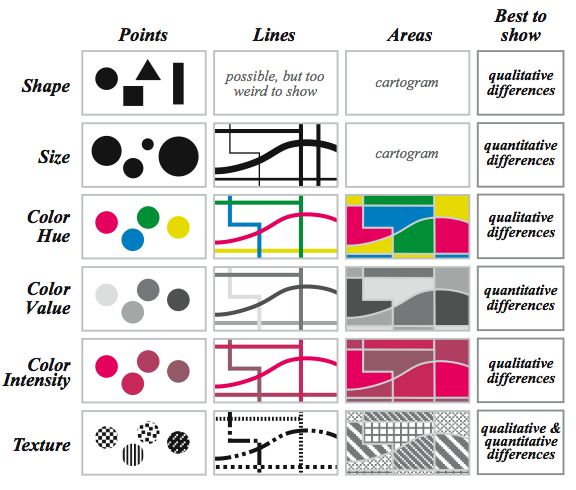
\includegraphics[width=.7\textwidth]{figures/intro/retinal_variables.png}
        \caption{This tabular form of Bertin's retinal variables is from Understanding Graphics \cite{malamedInformationDisplayTips2010} who reproduced it from Krygier and Wood's \textit{Making Maps: A Visual Guide to Map Design for GIS}\cite{krygierMakingMapsVisual2005}}
    \end{figure}
\end{frame}

\begin{frame}{Visualizations are (mostly) evaluated on equivariance}
    \begin{description}
        \item[Expressiveness] structure preserving mappings from data to graphic (Mackinlay \cite{mackinlayAutomatingDesignGraphical1986})
        \item[Effectiveness] design choices made in deference to perceptual saliency (Mackinlay \cite{clevelandResearchStatisticalGraphics1987,clevelandGraphicalPerceptionTheory1984,chambersGraphicalMethodsData1983a, munznerVisualizationAnalysisDesign2014})
        \item[Naturalness] easier to understand when properties match (Norman \cite{norman_things_smart})
        \item[Graphical Integrity] graphs show \textbf{only} the data (Tufte \cite{tufteVisualDisplayQuantitative2001})
    \end{description}
\end{frame}


\begin{frame}{Visualization is commutative maps}

    \pause
    %% deconstruct D\R\V
    \begin{center}
        \textbf{Tam: Add topology and make it functional}
    \end{center}
\end{frame}

\begin{frame}{Models describe composition}
    \begin{description}
        \item[language model] APT, GoG: syntax, semantics, and grammar of graphics (Mackinlay, Wilkenson  \cite{mackinlayAutomatingDesignGraphical1986, mackinlayAUTOMATICDESIGNGRAPHICAL1987,wilkinsonGrammarGraphics2005})
        \item[functional dependencies] constrained maps between data and visual representation(Sugibuchi \cite{sugibuchiFramwork2009}) 
        \item[category theory] the semiotics of visualization are commutative (Vickers \cite{vickersUnderstandingViz2013})
        \item[algebraic process] data ($\alpha$) and viz ($\omega$) transforms are symmetric (Kindlmann and Scheidegger \cite{kindlmannAlgebraicProcessVisualization2014})
        \begin{columns}
            \column{.5\textwidth}
       
            \begin{description}
                \item[D] data 
                \item[R] representations
                \item[V] visualizations
            \end{description}
            \column{.5\textwidth}
            \begin{equation*}
                \begin{tikzcd}[ampersand replacement=\&]
                    D \arrow[d, "\alpha"'] \arrow[r, "r_1"] \& R \arrow[r, "\nu"]  \& V \arrow[d, "\omega"] \\
                    D \arrow[r, "r_2"']                     \& R \arrow[r, "\nu"'] \& V                    
                \end{tikzcd}
                \end{equation*}
       
        \end{columns} 
     
    \end{description}
\end{frame}


\begin{frame}{Mathematical Frameworks for evaluating visualization}
    \begin{enumerate}
        \item APT: visualization has syntax and semantics like a language  (Mackinlay  \cite{mackinlayAutomatingDesignGraphical1986, mackinlayAUTOMATICDESIGNGRAPHICAL1987})
        \item visualization has functional dependencies that can be represented as graphs (Sugibuchi \cite{sugibuchiFramwork2009}) 
        \item the semiotics of visualization are commutative in a category theory framework (Vickers \cite{vickersUnderstandingViz2013})
        \item data ($\alpha$) and viz ($\omega$) symmetries (Kindlmann and Scheidegger \cite{kindlmann2014algebraic})
        \begin{block}{$v\circ r_2 \circ \alpha =\omega\circ v\circ r_1$}
            \begin{equation*}
            \begin{tikzcd}[ampersand replacement=\&]
                D \arrow[d, "\alpha"'] \arrow[r, "r_1"] \& R \arrow[r, "\nu"]  \& V \arrow[d, "\omega"] \\
                D \arrow[r, "r_2"']                     \& R \arrow[r, "\nu"'] \& V                    
            \end{tikzcd}
            \end{equation*}
        \end{block}
\end{frame}


\begin{frame}{Structure is encoded in variables and continuity}
    \begin{figure}
        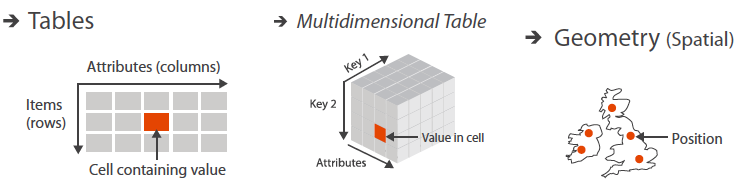
\includegraphics[width=1\textwidth]{figures/intro/munzner_datatypes.png}
        \caption{Image is figure 2.8 in Munzner's Visualization Analysis and Design\cite{munznerVisualizationAnalysisDesign2014}}
    \end{figure}
    \begin{description}
        \item[binding] metadata are structural \textit{keys} with associated \textit{values} (Munzner \cite{munznerVisualizationAnalysisDesign2014})] 
        \item[continuity])
        \item[variables] Fibers can hold schema like encodings of variables (Spivak \cite{spivakDatabasesAreCategories2010,spivakSIMPLICIALDATABASES})
    \end{description}
\end{frame}


begin{frame}{Monoid Actions: Permutation}
    \begin{figure}
        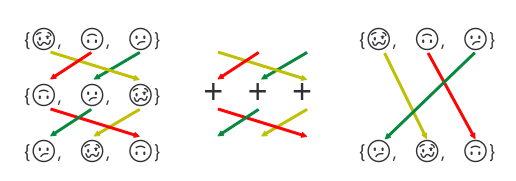
\includegraphics[width=1\linewidth]{figures/math/monoid_emoji.png}
    \end{figure}
\end{frame}

\begin{frame}{Why monoids? partial orders}
    \begin{figure}
        \begin{overprint}
            \onslide<1|handout:0>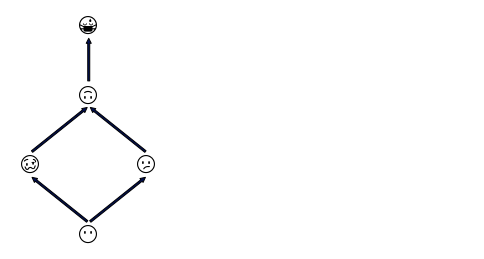
\includegraphics[width=1\linewidth]{figures/math/monoid_hasse.png}
            \onslide<2|handout:0>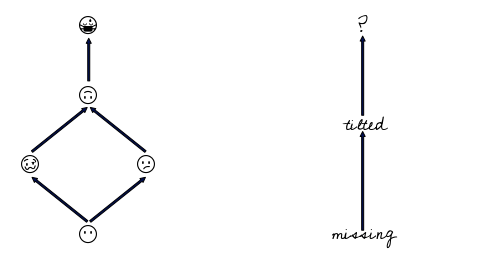
\includegraphics[width=1\linewidth]{figures/math/monoid_monotone.png}
            \onslide<3>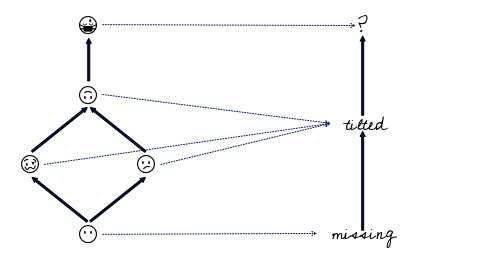
\includegraphics[width=1\linewidth]{figures/math/monoid_maps.png}
        \end{overprint}
    \caption{Inspired by definition 1.59 diagram in Spivak and Fong's An Invitation to Applied Category Theory \cite{fongInvitationAppliedCategory2019}}
    \end{figure}
\end{frame}

%appendix 
\begin{frame}{\dbase\ is an indexing space independent of component semantics}
    \begin{equation}
        \pi:\dtotal_1\oplus\ldots\oplus \dtotal_i \oplus\ldots \oplus \dtotal_n \rightarrow \dbase
    \end{equation}
\end{frame}




%rename so everything is consistent


